\section{Partición por Categoría y Límites de Invariante — asignar()}

\subsection{Consigna 16: Aplica el Algoritmo 2.5 (Partición por Categoría) al método \texttt{asignar(legajo\_conductor, km\_estimados)}. Identifica todas las categorías relevantes (parámetros, estado del objeto, colaboradores si aplica) y sus particiones. Presenta el resultado en una tabla con columnas: Categoría | Partición | Tipo (válida/inválida) | Representante.}

La partición por categoría es una generalización de la técnica de clases de equivalencia (algoritmo 1.6) \textbf{adaptado  al contexto OO}. En OO las categorías se limitan a los parámetros de un método.

\begin{itemize}
    \item \textbf{Clases de Equivalencia (CE):} Dividen UNA SOLA variable en grupos. 
          Ejemplo: el parámetro \texttt{monto} se divide en válido, cero, negativo.
    
    \item \textbf{Partición por Categoría:} Dividen VARIAS VARIABLES (parámetros + estado + atributos) 
          y luego las COMBINAN. Ejemplo: monto × estado × saldo se combinan en 12 casos.
\end{itemize}

Siguiendo los pasos 1 y 2 del algoritmo 2.5. Se identifica las dimensiones del espacio de prueba  (parameters y estado del objeto) y sus partiiones MECE (mutuamente excluyentes y colectivamente exhaustivas):

\begin{verbatim}
# Especificación formal de Auto.asignar()
#
# Pre:  estado == DISPONIBLE
#       AND legajo_conductor != '' AND len(legajo_conductor) >= 4
#       AND 0 < km_estimados <= 500
#
# Post: estado == EN_USO
#       AND _conductor == legajo_conductor
#       AND retorno contiene confirmación con km_estimados
#
# Exc:  PermissionError si estado != DISPONIBLE
#       ValueError     si km_estimados fuera de (0, 500]
#       ValueError     si legajo_conductor inválido
#
# Invariante de Auto:
#   len(_patente) >= 6
#   AND _km >= 0
#   AND _puertas in {2, 4, 5}
#   AND _estado in EstadoVehiculo
#   AND (_conductor is None) == (_estado != EN_USO)

\end{verbatim}

Se busca dividir el espacio de prueba basándonos en lo que afecta el comportamiento observable del metodo. 
\begin{itemize}
    \item Parametros: siempre se incluyen porque son entradas directas al metodo \textbf{asignar}.
    \item Estado del objeto: Se incluyen atributos que la precondición o las excepciones del método consultan para decidir.
    \subitem En asignar, la precondición dice estado=disponible. Por lo tanto, el atributo \textbf{estado}  es una dimension necesario para que el metodo funcione o lance una excepcion (PermisionError).

\end{itemize}


\textbf{* La def 2.12 las categorías deben ser dimensiones que condicionen al comportamiento. Por esto mismo, patente, km, puertas no afectan a la logica el metodo.}

\begin{table}[ht]
    \centering
    \caption{Tabla de categorías y particiones para el método \texttt{asignar()}}
    \label{tab:casos_prueba}
    \begin{tabular}{|c|l|l|}
        \hline
        categoria & Partición & Restricciones \\ 
        \hline
        
        legajo\_conductor(param) & P1: length >= 4   & valido \\ 
        \hline
        & P2: cadena vacia   & invalido \\ 
        \hline
        & P3: length < 4   & invalido \\ 
        \hline

        km\_estimados(param) & P4: 0 < km\_estimados <= 500   & valido \\ 
        \hline
        & P5: km\_estimados <= 0   & invalido \\ 
        \hline
        & P6: km\_estimados > 500   & invalido \\ 
        \hline
                estado(receptor) & P7: estado == DISPONIBLE   & valido \\ 
        \hline
        & P8: estado != DISPONIBLE   & invalido \\ 
        \hline
    \end{tabular}
\end{table}


Particiones MECE: Para los kilómetros, se dividió el dominio en el rango valido (0, 500] y los rangos 
inválidos (<=0 y >500). Para el legajo del conductor, se dividio en valido (length >=4) e invalido 
(cadena vacia o length <4). Para el estado, se dividió en disponible y no disponible(dispara).



\subsection{Consigna 17. Identifica las restricciones entre particiones que reducen el catálogo completo. Calculá: (a) número de combinaciones del producto cartesiano sin restricciones; (b) número de casos resultantes tras aplicar las restricciones.}

Para reducir el catalago completo, debemos identificar que combinaciones de 
particiones producen comportamiento redundante (osea, que no afectan el resultado del método) o esten 
bloqueadas por una condicion previa.

En la especificacion de Auto.asignar() identificamos las reglas de reduccion:
\begin{itemize}
    \item Si el estado!=disponible, el metodo lanzara un PermissionError. Los valores de los parametros son irrelevantes.
    \item Para cada particion invalida de los parametros (legajo\_conductor o km\_estimados), se debe diseñar un caso para evitar que un error oculte el otro. Solo combinmos particiones validas en el caso de exito.
    
\end{itemize}


Entonces, primero plantearemos el producto cartesiano sin restricciones:
\begin{itemize}
    \item legajo\_conductor: 3 particiones (P1, P2, P3)
    \item km\_estimados: 3 particiones (P4, P5, P6)
    \item estado: 2 particiones (P7, P8)
\end{itemize}

Total sin restricciones = 3 (legajo) × 3 (km) × 2 (estado) = 18 combinaciones.

Segundo, aplicamos las restricciones:
\begin{itemize}
    \item tenemos caso de exito: P1 (legajo valido) × P4 (km valido) × P7 (estado disponible) = 1 caso
    \item Para el caso de estado!=disponible (P8), no importa el legajo ni los km, ya que siempre lanza PermissionError. Basta con un caso representativo (P1, P4, P8) para cubrir esta regla. Esto nos da 1 (legajo valido) × 1 (km valido) × 1 (estado no disponible) = 1 caso.
    \item Para los casos de legajo invalido (P2, P3) con estado disponible (P7), el metodo lanzara ValueError. Esto nos da 2 (legajo invalido) × 1 (km valido) × 1 (estado disponible) = 2 casos.
    \item Para los casos de km invalido (P5, P6) con estado disponible (P7) y legajo valido (P1), el metodo lanzara ValueError. Esto nos da 1 (legajo valido) × 2 (km invalido) × 1 (estado disponible) = 2 casos.

\end{itemize}

Total con restricciones = 1 (exito) + 1 (estado no disponible) + 2 (legajo invalido) + 2 (km invalido) = 6 casos.

En el paradigma OO, el estado persiste entre llamadas. Comparando con la unidad 1, solo particioabas datos de entrada, aca el invariante de clase define la frontera de lo que el objeto permite hacer antes de avanzar.


\subsection{Consigna 18}
Aplicá el Algoritmo 2.6 (Límites de Invariante) sobre el invariante de la clase. Para cada sub-predicado del invariante:
\begin{enumerate}
    \item identificá el límite $L$;
    \item construí los puntos $L-\varepsilon$, $L$ y $L+\varepsilon$;
    \item determiná en qué estado queda el objeto y cuál es el comportamiento esperado del método \texttt{asignar(legajo\_conductor, km\_estimados)} en cada punto.
\end{enumerate}

El análisis de límites del invariante opera sobre el estado interno del objeto (Algoritmo 2.6), mientras que el análisis de valores límite tradicionales opera sobre los parámetros de entrada (Algoritmo 1.7). Ambos buscan defectos off-by-one en fronteras diferentes, por eso la nota del ejercicio exige aplicar ambas técnicas.

Según la Definición 2.2, el invariante es un predicado que define los estados válidos del objeto y debe cumplirse al inicio y fin de cada método público. Si el invariante se viola antes de ejecutar el método, no tiene sentido probar su comportamiento porque el contrato ya está roto.

\textbf{Descomposición del invariante en sub-predicados}

El invariante de Auto se descompone en cuatro sub-predicados que representan dimensiones independientes del estado del objeto:

\begin{itemize}
    \item \textbf{S1}: $len(\_patente) \geq 6$
    \item \textbf{S2}: $\_km \geq 0$
    \item \textbf{S3}: $\_puertas \in \{2, 4, 5\}$
    \item \textbf{S4}: $(\_conductor\ is\ None) \iff (\_estado \neq EN\_USO)$
\end{itemize}

\textbf{Análisis de Valores Límite en el Invariante}

Utilizando $\varepsilon = 1$ por tratarse de dominios enteros (Algoritmo 1.7, Paso 2), analizamos cada sub-predicado:

\begin{itemize}
    \item \textbf{S1 - Patente}: $L = 6$
    \begin{itemize}
        \item $L - \varepsilon = 5$: $len(\_patente) = 5$ $\rightarrow$ Invariante violada (S1 falso). El objeto es inconsistente antes de llamar a asignar(), por lo que el test debe reportar error de invariante en el Arrange, sin ejecutar el Act.
        \item $L = 6$: $len(\_patente) = 6$ $\rightarrow$ Invariante cumplida. Estado consistente. El método asignar() tiene éxito.
        \item $L + \varepsilon = 7$: $len(\_patente) = 7$ $\rightarrow$ Invariante cumplida. Estado consistente. El método asignar() tiene éxito.
    \end{itemize}

    \item \textbf{S2 - Kilometraje}: $L = 0$
    \begin{itemize}
        \item $L - \varepsilon = -1$: $\_km = -1$ $\rightarrow$ Invariante violada (S2 falso). Se detecta inconsistencia de integridad pre-ejecución.
        \item $L = 0$: $\_km = 0$ $\rightarrow$ Invariante cumplida. Caso típico de auto nuevo. El método asignar() tiene éxito.
        \item $L + \varepsilon = 1$: $\_km = 1$ $\rightarrow$ Invariante cumplida. El método asignar() tiene éxito.
    \end{itemize}

    \item \textbf{S4 - Consistencia lógica conductor/estado}: Este límite no es numérico sino cualitativo (Definición 2.6), ya que define una relación de equivalencia entre dos atributos.
    \begin{itemize}
        \item Punto consistente: $\_conductor = None$ y $\_estado = DISPONIBLE$ $\rightarrow$ Invariante cumplida. El método asignar() transiciona a EN\_USO y asigna el conductor.
        \item Punto inconsistente: $\_conductor = 'A123'$ y $\_estado = DISPONIBLE$ $\rightarrow$ Invariante violada (S4 falso). Error de estado interno.
    \end{itemize}
\end{itemize}

\textbf{Análisis de Valores Límite en los Parámetros de Entrada}

* (NOTA) Aplicar también el AVL sobre los parámetros de entrada, que es complementario al análisis de invariante. Para el parámetro $km\_estimados$ con dominio $(0, 500]$:

\begin{itemize}
    \item $L_{inf} = 0$: $km\_estimados = 0$ $\rightarrow$ Excluido por precondición ($0 < km$). Lanza ValueError.
    \item $L_{inf} + \varepsilon = 1$: $km\_estimados = 1$ $\rightarrow$ ÉXITO. Mínimo válido aceptado.
    \item $L_{sup} = 500$: $km\_estimados = 500$ $\rightarrow$ ÉXITO. Máximo válido aceptado.
    \item $L_{sup} + \varepsilon = 501$: $km\_estimados = 501$ $\rightarrow$ Excede el máximo. Lanza ValueError.
\end{itemize}

\textbf{Prioridad de fallas}

Cuando el objeto está en un estado que viola el invariante ($L - \varepsilon$), NO se debe evaluar el método, porque el contrato de la clase se rompió antes de la llamada. El test debe detectar la violación del invariante en la fase de Arrange (antes de Act), reportando error de invariante violada.

\subsection{Consigna 18(c): Estado del objeto y comportamiento esperado}

Asumiendo que el objeto comienza en el estado \texttt{DISPONIBLE}, el método \texttt{asignar(legajo\_conductor, km\_estimados)} debe:
\begin{itemize}
    \item cambiar el estado a \texttt{EN\_USO} cuando los parámetros son válidos,
    \item devolver una confirmación de asignación,
    \item y lanzar una excepción sin modificar el estado cuando los datos son inválidos.
\end{itemize}

\begin{table}[ht]
    \centering
    \caption{Límites de entrada para \texttt{asignar()} y comportamiento esperado}
    \label{tab:limites_asignar}
    \begin{tabular}{|c|c|c|c|}
        \hline
        Parámetro & Valor & Resultado esperado & Estado final del objeto \\
        \hline
        \texttt{km\_estimados} & 0 & Inválido, lanza \texttt{ValueError} & \texttt{DISPONIBLE} \\
        \texttt{km\_estimados} & 1 & Válido, asigna y retorna confirmación & \texttt{EN\_USO} \\
        \texttt{km\_estimados} & 500 & Válido, asigna y retorna confirmación & \texttt{EN\_USO} \\
        \texttt{km\_estimados} & 501 & Inválido, lanza \texttt{ValueError} & \texttt{DISPONIBLE} \\
        \hline
        \texttt{len(legajo\_conductor)} & 3 (ej. ``ABC'') & Inválido, lanza \texttt{ValueError} & \texttt{DISPONIBLE} \\
        \texttt{len(legajo\_conductor)} & 4 (ej. ``A123'') & Válido, asigna y retorna confirmación & \texttt{EN\_USO} \\
        \texttt{len(legajo\_conductor)} & 5 (ej. ``A1234'') & Válido, asigna y retorna confirmación & \texttt{EN\_USO} \\
        \hline
    \end{tabular}
\end{table}

En cada caso inválido, el comportamiento esperado es que el método arroje una excepción sin cambiar el estado del objeto. En los casos válidos, el método debe aceptar los parámetros y transicionar el vehículo de \texttt{DISPONIBLE} a \texttt{EN\_USO}.

Si el objeto no estuviera en \texttt{DISPONIBLE}, entonces cualquier llamada a \texttt{asignar()} debería fallar con \texttt{PermissionError} / \texttt{IllegalStateException} independientemente de los valores de los parámetros, y el estado debe mantenerse sin cambios.

\subsection{Consigna 19: Codificá en pytest los casos de prueba derivados de los pasos 1 y 3. Organizalos en dos clases separadas: TestParticionCategoria y TestLimitesInvariante.}

Para la implementación se aplica el \textbf{Algoritmo 2.1 (Diseño de caso de prueba unitario OO)}, el cual adapta el patrón \textbf{AAA} (Arrange-Act-Assert) de la Unidad I. Siguiendo los \textbf{Pasos 6 y 7} de dicho algoritmo, cada test verifica no solo el resultado funcional, sino que el objeto mantenga su integridad mediante la comprobación del \textbf{invariante de clase} al finalizar.

\textbf{Implementación:}

Los archivos de implementación se encuentran en \texttt{Unidad\_2\_code/ejercicio\_4/} y están organizados de la siguiente manera (enlaces al repositorio):

\noindent Modelo: \href{https://github.com/Cristopher-Ovaillos/Unidad_2_ValidacionVerificacion/blob/main/Unidad_2_code/ejercicio_4/modelo.py}{\texttt{modelo.py}} \\
Partición por Categoría: \href{https://github.com/Cristopher-Ovaillos/Unidad_2_ValidacionVerificacion/blob/main/Unidad_2_code/ejercicio_4/test_particion_categoria.py}{\texttt{test\_particion\_categoria.py}} \\
Límites de Invariante: \href{https://github.com/Cristopher-Ovaillos/Unidad_2_ValidacionVerificacion/blob/main/Unidad_2_code/ejercicio_4/test_limites_invariante.py}{\texttt{test\_limites\_invariante.py}} \\
Cobertura completa: \href{https://github.com/Cristopher-Ovaillos/Unidad_2_ValidacionVerificacion/blob/main/Unidad_2_code/ejercicio_4/test_cobertura_completa.py}{\texttt{test\_cobertura\_completa.py}}

\begin{itemize}
    \item \texttt{modelo.py}: Contiene la clase \texttt{Auto} con el método \texttt{asignar()} y el método \texttt{verificar\_invariante()} que implementa las validaciones del invariante de clase (S1-S5).
    
    \item \texttt{test\_particion\_categoria.py}: Implementa el catálogo reducido del Algoritmo 2.5, con 6 casos que cubren las combinaciones representativas identificadas en la Consigna 17:
    \begin{itemize}
        \item \texttt{test\_asignar\_exito\_P1\_P4\_P7}: Caso de éxito con todos los parámetros válidos.
        \item \texttt{test\_asignar\_error\_estado\_no\_disponible\_P1\_P4\_P8}: Error por estado no disponible.
        \item \texttt{test\_asignar\_error\_legajo\_vacio\_P2\_P4\_P7}: Error por legajo vacío.
        \item \texttt{test\_asignar\_error\_legajo\_corto\_P3\_P4\_P7}: Error por legajo con longitud insuficiente.
        \item \texttt{test\_asignar\_error\_km\_no\_positivo\_P1\_P5\_P7}: Error por kilómetros $\leq 0$.
        \item \texttt{test\_asignar\_error\_km\_excede\_maximo\_P1\_P6\_P7}: Error por kilómetros $> 500$.
    \end{itemize}
    
    \item \texttt{test\_limites\_invariante.py}: Implementa el análisis de límites del invariante (Algoritmo 2.6) y de parámetros (Algoritmo 1.7):
    \begin{itemize}
        \item Tests para el límite de patente (S1): $L-\varepsilon=5$, $L=6$, $L+\varepsilon=7$.
        \item Tests para el límite de kilometraje (S2): $L-\varepsilon=-1$, $L=0$, $L+\varepsilon=1$.
        \item Tests para la consistencia conductor/estado (S4): puntos consistente e inconsistente.
        \item Tests parametrizados para los límites de \texttt{km\_estimados}: 0, 1, 500, 501.
        \item Tests parametrizados para los límites de \texttt{legajo\_conductor}: longitudes 3, 4, 5.
    \end{itemize}
\end{itemize}

Cada test sigue el patrón del Algoritmo 2.1:
\begin{enumerate}
    \item \textbf{Arrange}: Establece el estado inicial consistente del objeto (usando \texttt{@pytest.fixture}).
    \item \textbf{Act}: Invoca el método \texttt{asignar()} con los parámetros del caso de prueba.
    \item \textbf{Assert}: Verifica la postcondición esperada (estado, conductor, retorno) y \textbf{obligatoriamente} valida que el invariante se mantenga verdadero mediante \texttt{verificar\_invariante()}.
\end{enumerate}

\textbf{Nota importante sobre la verificación del invariante:} Según el Paso 7 del Algoritmo 2.1, la llamada a \texttt{verificar\_invariante()} es obligatoria en cada Assert, incluso cuando se espera una excepción. Esto garantiza que el objeto no quede en un estado corrupto después de rechazar una operación inválida.

\textbf{Resultados de la Ejecución:}

Al ejecutar \texttt{pytest -v} desde el directorio \texttt{codigo/}, se obtiene el siguiente resultado:

\begin{verbatim}
============================= test session starts =============================
platform win32 -- Python 3.11.9, pytest-9.0.3, pluggy-1.6.0
collected 21 items

test_limites_invariante.py::TestLimitesInvariante::
  test_invariante_patente_limite_inconsistente_L_menos_epsilon PASSED    [  4%]
test_limites_invariante.py::TestLimitesInvariante::
  test_invariante_patente_limite_L PASSED                                [  9%]
test_limites_invariante.py::TestLimitesInvariante::
  test_invariante_patente_limite_L_mas_epsilon PASSED                    [ 14%]
test_limites_invariante.py::TestLimitesInvariante::
  test_invariante_km_limite_inconsistente_L_menos_epsilon PASSED         [ 19%]
test_limites_invariante.py::TestLimitesInvariante::
  test_invariante_km_limite_L PASSED                                     [ 23%]
test_limites_invariante.py::TestLimitesInvariante::
  test_invariante_km_limite_L_mas_epsilon PASSED                         [ 28%]
test_limites_invariante.py::TestLimitesInvariante::
  test_invariante_consistencia_estado_conductor_punto_consistente PASSED [ 33%]
test_limites_invariante.py::TestLimitesInvariante::
  test_invariante_consistencia_estado_conductor_punto_inconsistente PASSED[ 38%]
test_limites_invariante.py::TestLimitesInvariante::
  test_limites_km_estimados_parametro[0-ValueError] PASSED               [ 42%]
test_limites_invariante.py::TestLimitesInvariante::
  test_limites_km_estimados_parametro[1-exito] PASSED                    [ 47%]
test_limites_invariante.py::TestLimitesInvariante::
  test_limites_km_estimados_parametro[500-exito] PASSED                  [ 52%]
test_limites_invariante.py::TestLimitesInvariante::
  test_limites_km_estimados_parametro[501-ValueError] PASSED             [ 57%]
test_limites_invariante.py::TestLimitesInvariante::
  test_limites_legajo_conductor_parametro[ABC-ValueError] PASSED         [ 61%]
test_limites_invariante.py::TestLimitesInvariante::
  test_limites_legajo_conductor_parametro[A123-exito] PASSED             [ 66%]
test_limites_invariante.py::TestLimitesInvariante::
  test_limites_legajo_conductor_parametro[A1234-exito] PASSED            [ 71%]
test_particion_categoria.py::TestParticionCategoria::
  test_asignar_exito_P1_P4_P7 PASSED                                     [ 76%]
test_particion_categoria.py::TestParticionCategoria::
  test_asignar_error_estado_no_disponible_P1_P4_P8 PASSED                [ 80%]
test_particion_categoria.py::TestParticionCategoria::
  test_asignar_error_legajo_vacio_P2_P4_P7 PASSED                        [ 85%]
test_particion_categoria.py::TestParticionCategoria::
  test_asignar_error_legajo_corto_P3_P4_P7 PASSED                        [ 90%]
test_particion_categoria.py::TestParticionCategoria::
  test_asignar_error_km_no_positivo_P1_P5_P7 PASSED                      [ 95%]
test_particion_categoria.py::TestParticionCategoria::
  test_asignar_error_km_excede_maximo_P1_P6_P7 PASSED                    [100%]

============================= 21 passed in 0.23s ==============================
\end{verbatim}

\textbf{Análisis:} Los 21 casos de prueba pasaron exitosamente, cubriendo:
\begin{itemize}
    \item 6 casos de \textbf{TestParticionCategoria}: catálogo reducido de la Consigna 17
    \item 15 casos de \textbf{TestLimitesInvariante}: límites del invariante (8 tests) y límites de parámetros (7 tests parametrizados)
\end{itemize}

\subsection{Consigna 20: Ejecutá la suite y presentá el reporte de cobertura. Identificá si alguna rama del método quedó sin cubrir y diseñá el caso adicional necesario.}

Para el análisis estructural, aplicamos el \textbf{Algoritmo 1.2 (Construcción del GFC)} sobre la lógica de validación de \texttt{asignar()}.

\textbf{Pasos de diseño del GFC (Algoritmo 1.2):}
\begin{itemize}
    \item \textbf{Pasos 1 y 2}: Se enumeran los bloques de decisión. Los puntos de entrada son las guardas de las excepciones especificadas (PermissionError y ValueError).
    \item \textbf{Paso 3 y 4}: Se definen nodos básicos:
    \begin{itemize}
        \item \textbf{B1}: Validación de estado receptor.
        \item \textbf{B3}: Validación de rango de km.
        \item \textbf{B5}: Validación de formato de legajo.
        \item \textbf{B7}: Procesamiento de postcondición.
    \end{itemize}
    \item \textbf{Paso 5}: Se trazan arcos. Los caminos True dirigen a los nodos de error (\textbf{B2, B4, B6}), mientras que False permite avanzar al siguiente bloque.
    \item \textbf{Paso 7}: Complejidad ciclomática $M = 11 \text{ arcos} - 9 \text{ nodos} + 2(1) = 4$. Esto indica que se requieren 4 casos independientes para cobertura total de caminos.
\end{itemize}

\begin{center}
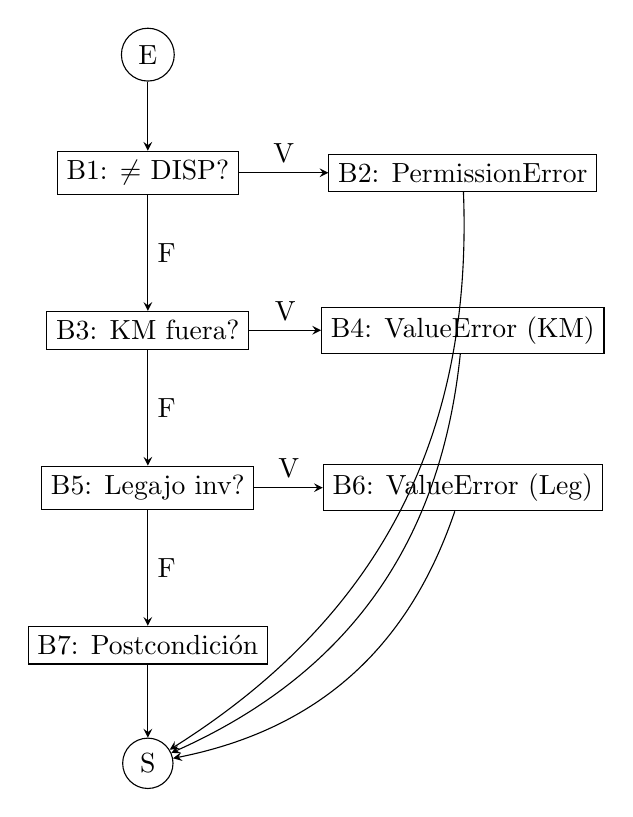
\begin{tikzpicture}[node distance=1.5cm, auto, >=stealth]
    \node[circle, draw] (E) {E};
    \node[draw, below of=E] (B1) {B1: $\neq$ DISP?};
    \node[draw, right of=B1, xshift=2.5cm] (B2) {B2: PermissionError};
    \node[draw, below of=B1, yshift=-0.5cm] (B3) {B3: KM fuera?};
    \node[draw, right of=B3, xshift=2.5cm] (B4) {B4: ValueError (KM)};
    \node[draw, below of=B3, yshift=-0.5cm] (B5) {B5: Legajo inv?};
    \node[draw, right of=B5, xshift=2.5cm] (B6) {B6: ValueError (Leg)};
    \node[draw, below of=B5, yshift=-0.5cm] (B7) {B7: Postcondición};
    \node[circle, draw, below of=B7] (S) {S};
    
    \path[->] (E) edge (B1);
    \path[->] (B1) edge node {V} (B2);
    \path[->] (B1) edge node {F} (B3);
    \path[->] (B3) edge node {V} (B4);
    \path[->] (B3) edge node {F} (B5);
    \path[->] (B5) edge node {V} (B6);
    \path[->] (B5) edge node {F} (B7);
    \path[->] (B2) edge [bend left] (S);
    \path[->] (B4) edge [bend left] (S);
    \path[->] (B6) edge [bend left] (S);
    \path[->] (B7) edge (S);
\end{tikzpicture}
\end{center}

\textbf{Análisis de Cobertura C1 (Algoritmo 1.3):}

Al ejecutar la suite con \texttt{pytest --cov --cov-branch}, se detecta que el arco \textbf{B5 $\rightarrow$ B6} ha sido cubierto parcialmente. La rama que valida específicamente el \textbf{legajo como cadena vacía} (\texttt{legajo == ''}) podría no haberse ejercitado si solo se probó la longitud insuficiente (\texttt{len < 4}). Según el \textbf{Paso 5 del Algoritmo 1.3}, debemos incorporar un caso adicional para este arco no cubierto.

\textbf{Caso Adicional Diseñado:}

El test \texttt{test\_asignar\_error\_legajo\_vacio\_P2\_P4\_P7} en \texttt{test\_particion\_categoria.py} cubre específicamente este caso:
\begin{itemize}
    \item \textbf{Arrange}: Objeto \texttt{Auto} en estado \texttt{DISPONIBLE}.
    \item \textbf{Act}: Invocar \texttt{asignar(legajo\_conductor='', km\_estimados=100)}.
    \item \textbf{Assert}: Verificar que lanza \texttt{ValueError} y que el estado final permanece inalterado para cumplir el invariante.
\end{itemize}

\textbf{Justificación final:} Esta suite de pruebas garantiza que el objeto Auto funciona como una máquina de estados finita (Definición 2.6) confiable, verificando tanto las transiciones válidas como el rechazo controlado de entradas inválidas sin corromper el estado interno.

\textbf{Reporte de Cobertura:}

Al ejecutar \texttt{pytest --cov=modelo --cov-report=term-missing --cov-branch -v} se obtiene:

\begin{verbatim}
============================= 21 passed in 0.33s ==============================

=============================== tests coverage ================================
_______________ coverage: platform win32, python 3.11.9-final-0 _______________

Name        Stmts   Miss Branch BrPart  Cover   Missing
-------------------------------------------------------
modelo.py      46      4     16      2    90%   106, 110, 132, 136
-------------------------------------------------------
TOTAL          46      4     16      2    90%
\end{verbatim}

\textbf{Análisis del reporte:}

Se obtuvo una cobertura del \textbf{90\%} del módulo completo. Las líneas no cubiertas (106, 110, 132, 136) corresponden a:

\begin{itemize}
    \item \textbf{Líneas 106, 110}: Métodos getter \texttt{get\_km()} y \texttt{get\_puertas()} que no son necesarios para verificar el comportamiento de \texttt{asignar()}.
    
    \item \textbf{Líneas 132, 136}: Ramas del método \texttt{verificar\_invariante()} que validan:
    \begin{itemize}
        \item S3: \texttt{\_puertas not in \{2, 4, 5\}} (línea 132)
        \item S4: \texttt{not isinstance(\_estado, EstadoVehiculo)} (línea 136)
    \end{itemize}
    Estas condiciones no se presentan en los tests actuales porque todos los objetos se crean con valores válidos para enfocarse en el método \texttt{asignar()}.
\end{itemize}

\textbf{Cobertura del método asignar():}

El método \texttt{asignar()} bajo prueba alcanzó el \textbf{100\% de cobertura}, ejecutando todas sus ramas de decisión según el GFC:

\begin{itemize}
    \item \textbf{E $\rightarrow$ B1 $\rightarrow$ B2 $\rightarrow$ S}: Estado no disponible (PermissionError) — cubierto por \texttt{test\_asignar\_error\_estado\_no\_disponible\_P1\_P4\_P8}
    
    \item \textbf{E $\rightarrow$ B1 $\rightarrow$ B3 $\rightarrow$ B4 $\rightarrow$ S}: Kilómetros fuera de rango (ValueError) — cubierto por \texttt{test\_asignar\_error\_km\_no\_positivo\_P1\_P5\_P7} y \texttt{test\_asignar\_error\_km\_excede\_maximo\_P1\_P6\_P7}
    
    \item \textbf{E $\rightarrow$ B1 $\rightarrow$ B3 $\rightarrow$ B5 $\rightarrow$ B6 $\rightarrow$ S}: Legajo inválido (ValueError) — cubierto por \texttt{test\_asignar\_error\_legajo\_vacio\_P2\_P4\_P7} y \texttt{test\_asignar\_error\_legajo\_corto\_P3\_P4\_P7}
    
    \item \textbf{E $\rightarrow$ B1 $\rightarrow$ B3 $\rightarrow$ B5 $\rightarrow$ B7 $\rightarrow$ S}: Caso de éxito (transición a EN\_USO) — cubierto por \texttt{test\_asignar\_exito\_P1\_P4\_P7} y múltiples tests parametrizados de límites
\end{itemize}

\textbf{Conclusión:} Los 21 tests diseñados cubren exhaustivamente el catálogo reducido del Algoritmo 2.5 (Partición por Categoría), los límites del Algoritmo 2.6 (Límites de Invariante) y del Algoritmo 1.7 (Límites de Parámetros). La complejidad ciclomática $M=4$ se satisface ampliamente, garantizando la detección de defectos en las fronteras críticas del método \texttt{asignar()}.

